A continuación se presentaran dos diagramas que grafican posibles interacciones
entre el sistema a desarrollar y personas o agentes externos, como sean los
clientes, los gerentes y los encargados de distintas áreas.

\subsubsection{Diagrama 1}
En este primer diagrama de contexto quedan reflejados los siguientes O-refinamientos:
\begin{enumerate}
\item Se implementa la página web y no las cajas de autoservicio. Esto además implica que el stock es manejado por la página web.
\item El encargado de entregas avisa por SMS y no mediante una llamada telefónica cuando esta por salir del depósito.
\item No se penaliza a los clientes cuando están ausentes al momento de la entrega.
\item Cuando un pedido no se puede entregar, éste vuelve al deposito.
\end{enumerate}

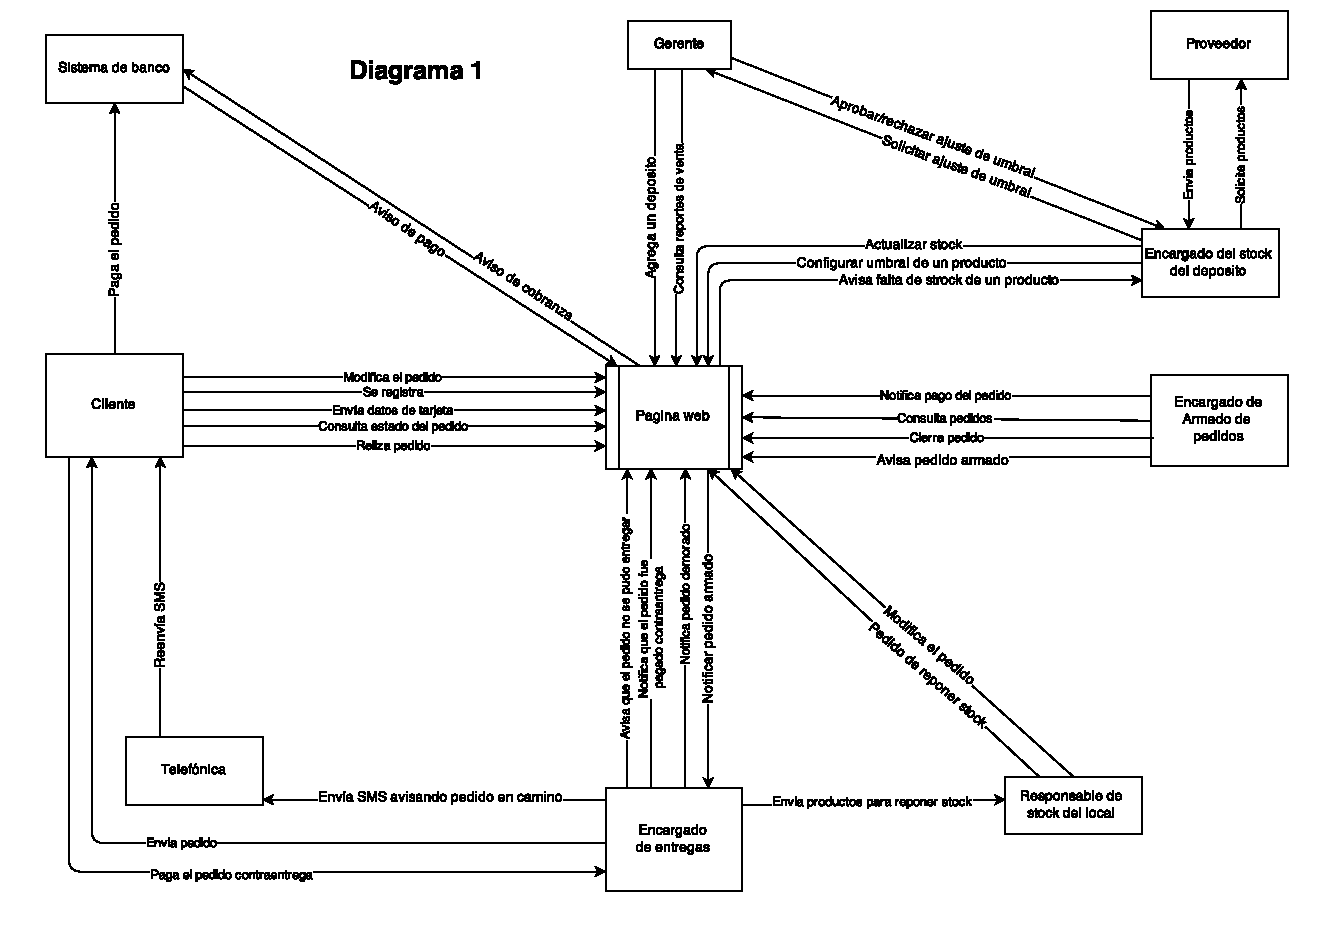
\includegraphics[angle=90]{diagrama1}

\subsubsection{Diagrama 2}
En este segundo diagrama de contexto, la página web mantiene registro de las compras online, que también incluye a los pedidos de reposición de stock de los locales. Por esta razón, en este diagrama de contexto el gerente también puede consultar las estadísticas de ventas, ya que éstas corresponden a las reposiciones de stock de los locales.

En este diagrama de contexto presentamos los siguientes O-refinamientos:
\begin{enumerate}
\item Se construyen las cajas de autoservicio para reducir las largas colas de los locales.
\item Las ventas que se realizan mediante las cajas de autoservicio no son registradas por la página web.
\item La pagina web administra el stock de los depósitos.
\item No existe un sistema para realizar pedidos online y, por lo tanto, tampoco un sistema de entrega de pedidos.	
\end{enumerate}

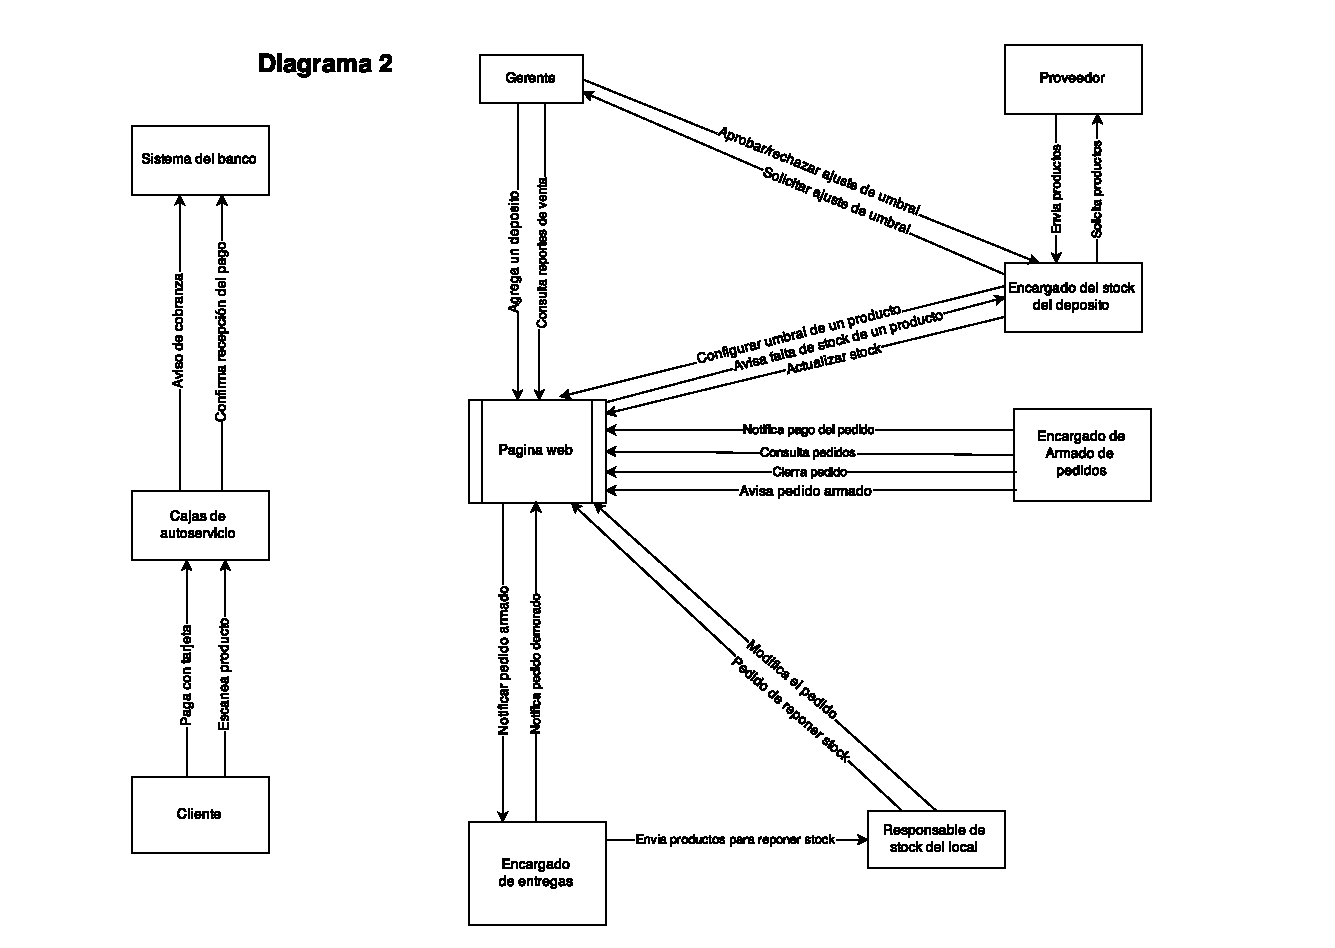
\includegraphics[angle=90]{diagrama2}

\subsubsection{Diagrama 3}
En este ultimo diagrama reflejamos un caso muy similar al primer diagrama, con la única diferencia de que aquí elegimos penalizar a los clientes cuando estos no se encuentran en su domicilio para recibir el pedido.\\
En este ultimo diagrama de contexto quedan reflejados los siguientes O-refinamientos:
\begin{enumerate}
\item Se implementa la página web y no las cajas de autoservicio. Esto además implica que el stock es manejado por la página web.
\item Se penaliza a los clientes cuando están ausentes al momento de la entrega.
\item Los pedidos de los clientes penalizados son rechazados por el sistema durante un tiempo X, definidor por el dueño.
\item Cuando un pedido no se puede entregar, éste vuelve al deposito.
\end{enumerate}

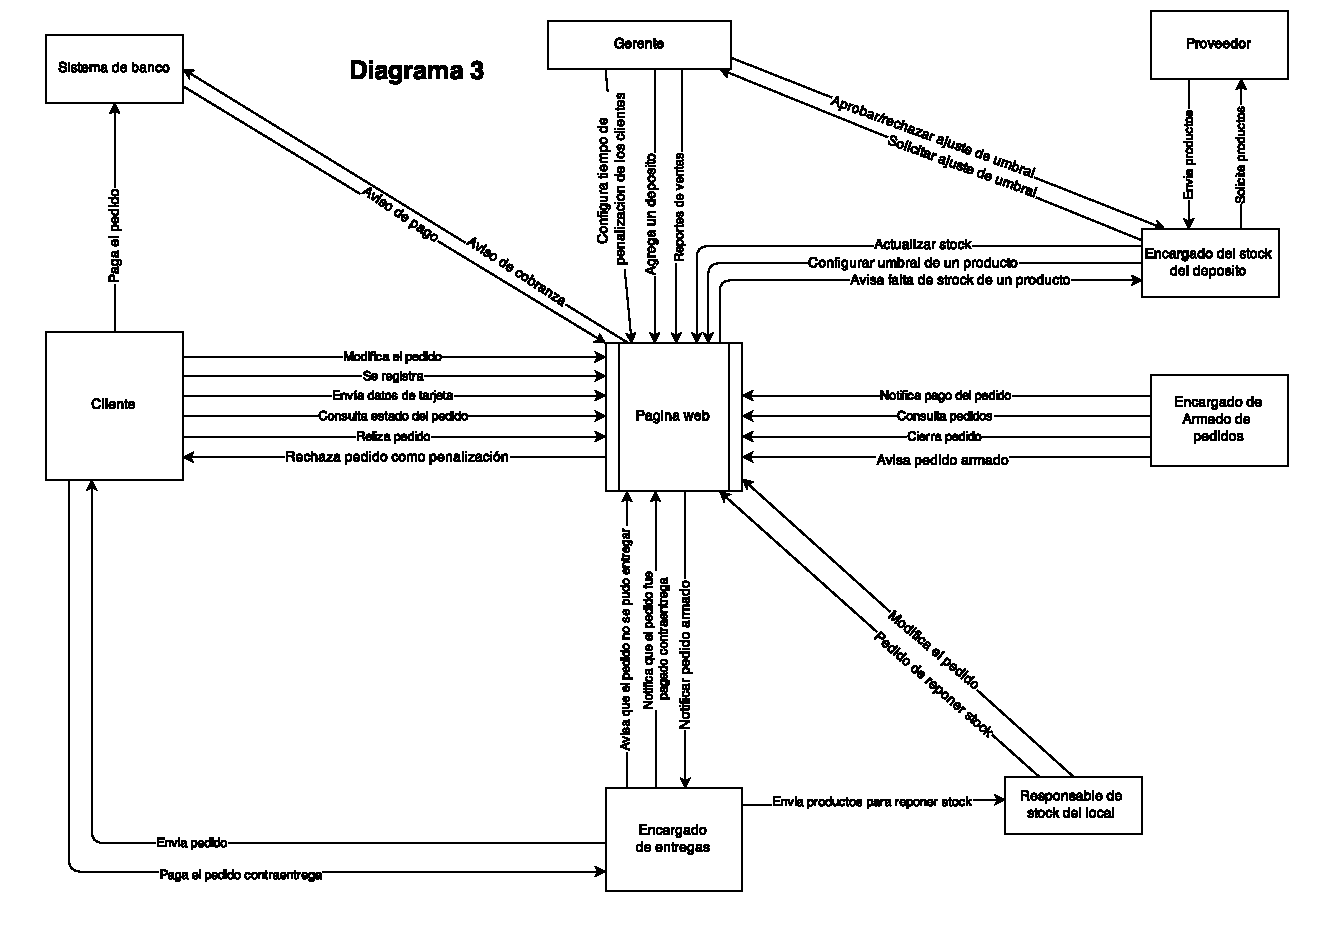
\includegraphics[angle=90]{diagrama3}